
\noindent\begin{minipage}{\textwidth}
    \begin{table}[H]
        \centering
        \caption{Hiperparâmetros e Resultados do Melhor Modelo - densenet\_v10\_BR\_opt\_aug}
        \vspace{0.2cm}
        \resizebox{\textwidth}{!}{%
            \begin{tabular}{ll | lrrr}
                \hline
                \multicolumn{2}{c|}{\textbf{Hiperparâmetros}} & \multicolumn{4}{c}{\textbf{Métricas por Classe}} \\ \hline
                \textbf{Parâmetro} & \textbf{Valor} & \textbf{Classe} & \textbf{Precisão} & \textbf{Recall} & \textbf{F1-Score} \\ \hline
    Agendador (Patience) & 3 & 31.2 & 0.6512 & 0.8829 & 0.7495 \\ 
Agendador de LR & ReduceLROnPlateau & 31.3 & 0.6872 & 0.6543 & 0.6703 \\ 
Architecture & densenet121 & 31.4 & 0.5992 & 0.6754 & 0.6351 \\ 
Batch Size & 32 & 32.3 & 0.8362 & 0.7831 & 0.8087 \\ 
Data Augmentation & False & 32.4 & 0.7241 & 0.5833 & 0.6462 \\ 
Decaimento de Peso (WD) & 0.0001 & 33.3 & 0.8010 & 0.7454 & 0.7722 \\ 
Dropout & 0.2747 & 41.4 & 0.8000 & 0.3404 & 0.4776 \\ 
Função de Perda & CrossEntropyLoss & 41.5 & 0.8824 & 0.6977 & 0.7792 \\ 
Hidden Units & 512 & 42.4 & 0.9474 & 0.5902 & 0.7273 \\ 
Label Smoothing & 0.1000 & 44.4 & 0.9615 & 0.7812 & 0.8621 \\ 
\cline{3-6} 
Otimizador & AdamW & \textbf{Média (Macro)} & 0.7694 & 0.7079 & 0.7279 \\ 
Taxa de Aprendizado (LR) & 3.26e-04 & \textbf{MCC} & \multicolumn{3}{c}{0.6930} \\ 
Unfreeze Layers & 5 &  & & &  \\ 
            \hline
            \end{tabular}%
        }
    \end{table}

    \begin{figure}[H]
        \centering
        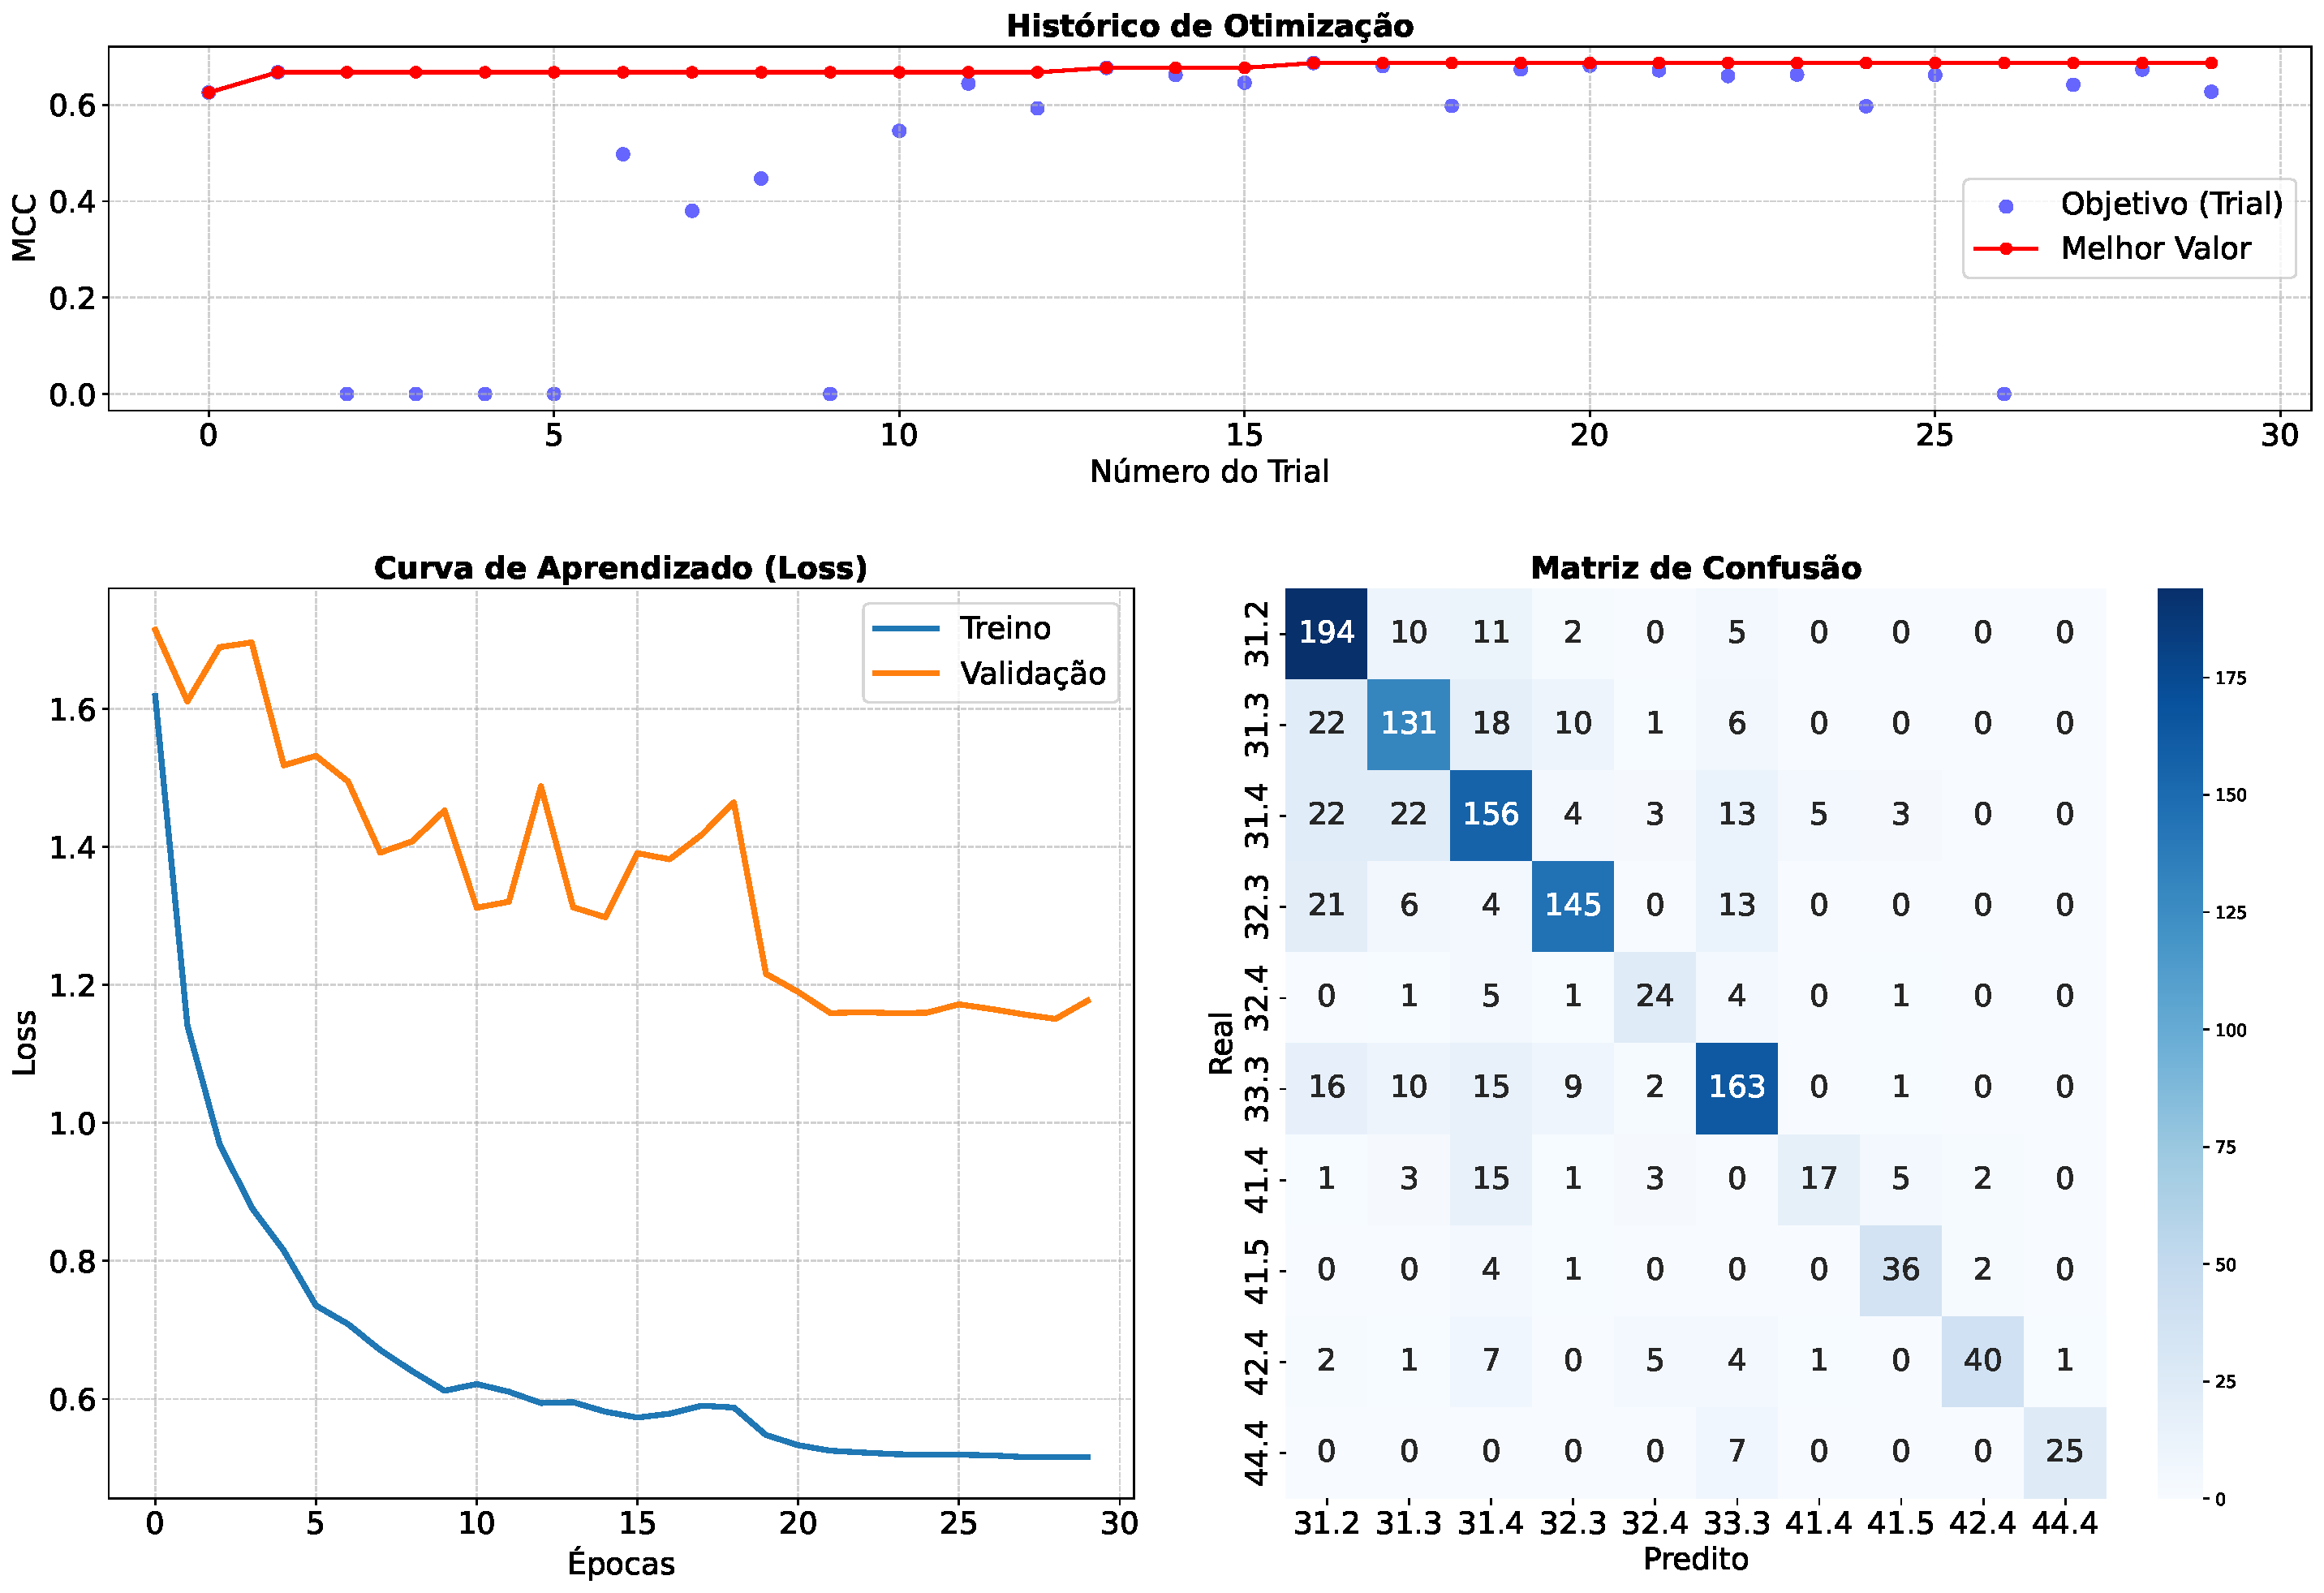
\includegraphics[width=0.85\textwidth]{tex/appendix/experiments/densenet_v10_BR_opt_aug/dashboard_consolidado.pdf}
        \caption{Histórico de Otimização, Curvas de Aprendizado e Matriz de Confusão - densenet\_v10\_BR\_opt\_aug}
    \end{figure}
\end{minipage}
\clearpage
